\chapter{理想弹塑性材料杆的有限元分析}
\label{cha:abaqus}
本章节使用商业有限元软件~ABAQUS~求解第~\ref{cha:ideal_theory}、第~\ref{cha:hardened}~章对应问题的数值解。自拟了一组参数,比较理论结果与计算结果,讨论二者的区别与联系。
\section{有限元模型的建立}
\subsection{有限元模型参数}
模型建立的基本参数见表~\ref{tab:abaqus}。
\begin{table}[htbp]
    \centering
    \caption{有限元建模参数}\label{tab:abaqus}
    \begin{tabular}{!{\vrule width 1.5pt}c|c|c|c|c|c!{\vrule width 1.5pt}}
    \noalign{\hrule height 1.5pt}
    杆长 & 半径 & 弹性模量 & 泊松比 & 屈服强度 & 扭转角 \\
    \hline
    $250~\text{mm}$ & $10~\text{mm}$ & $2.06\times10^5~\text{MPa}$ & $0.3$ & $235~\text{MPa}$ & $0.1~\text{rad}(5.73^\circ)$ \\
    \noalign{\hrule height 1.5pt}
    \end{tabular}
\end{table}
\subsection{网格划分}
模型采用拉伸实体建模,采用六面体单元、中性轴算法划分网格,模型网格划分情况如图~\ref{fig:mesh}~所示
\begin{figure}[htbp]
    \centering
	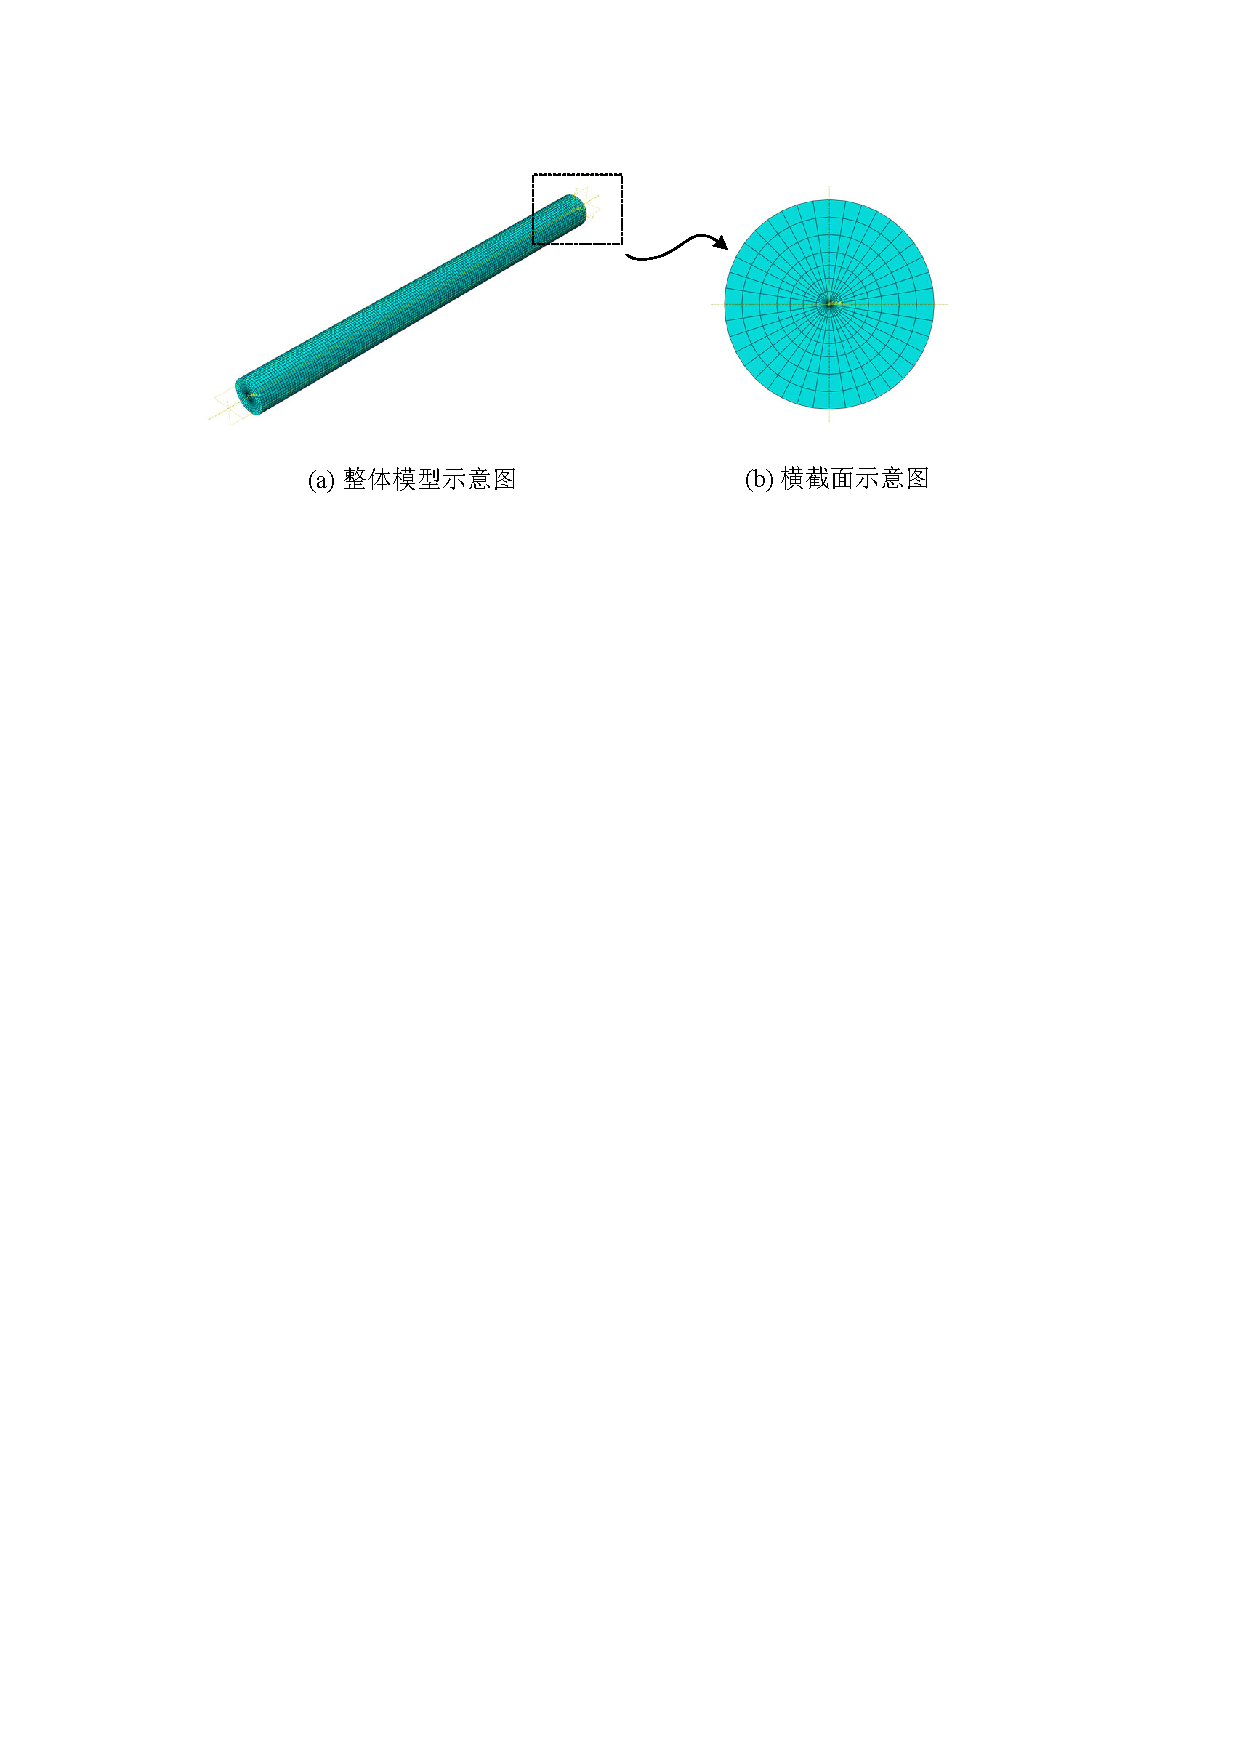
\includegraphics[width=0.7\textwidth]{mesh.pdf}
    \caption{网格划分}
    \label{fig:mesh}
\end{figure}
\subsection{加载过程模拟}
根据题目要求,有限元模型加载过程如下:

(1)在杆两侧截面中心分别设置参考点,并各自与端界面采用~coupling~约束绑定;

(2)分析步~1:将远端参考点完全固定定;

(3)分析步~2:近端参考点设置沿~Z~向的位移,大小为~0.2852~mm,使其全长全截面轴向应力均达到~{$f_y$};

(4)分析步~3:令近端参考点旋转~0.1~rad;

(5)提交作业,进行圆杆全加载过程有限元计算,并对结果进行对比分析。

\section{有限元分析结果}
圆杆~S33(即轴向力)应力云图,S23(即剪应力)应力云图和圆杆跨中截面正应力与剪应力分布云图如图所示如图~\ref{fig:ideal}~所示。
\begin{figure}[htbp]
    \centering
	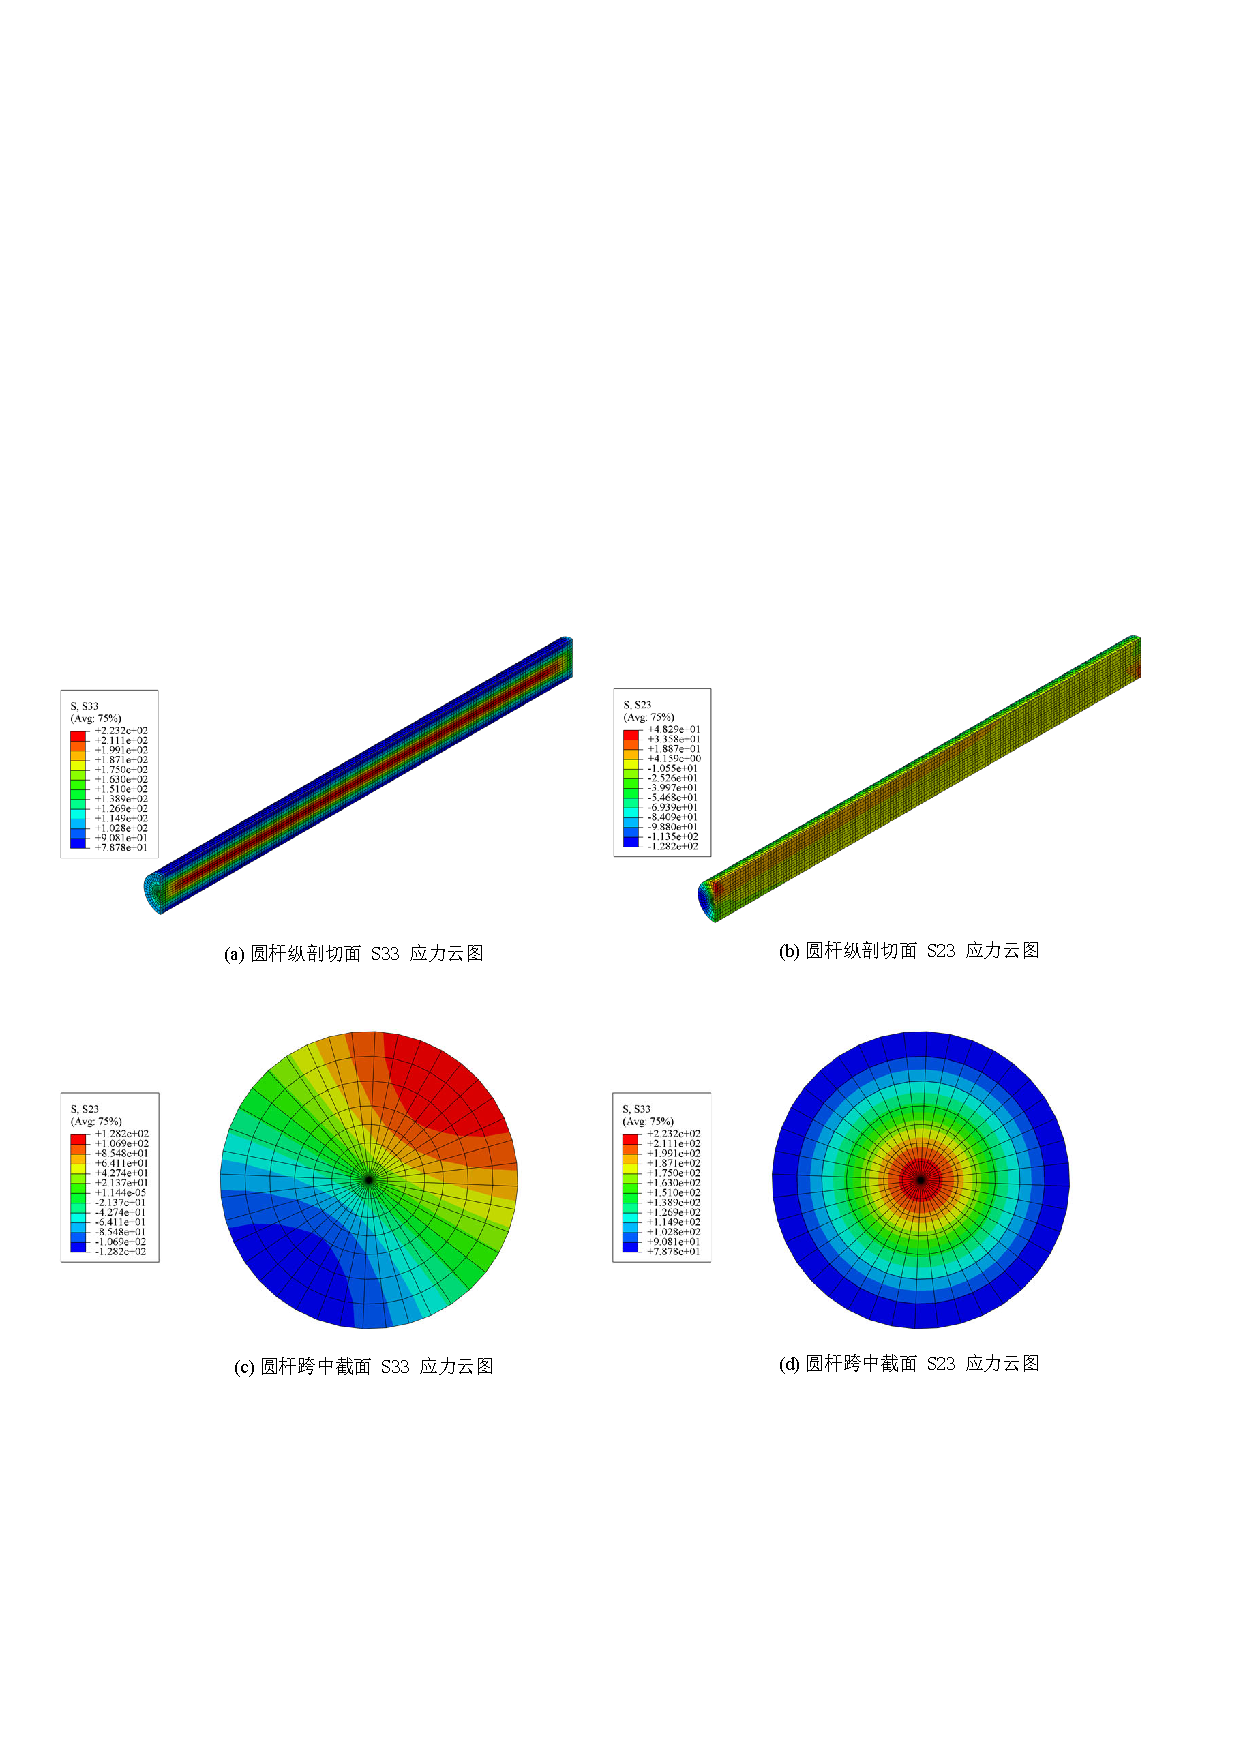
\includegraphics[width=1.0\textwidth]{ideal.pdf}
    \caption{理想弹塑性圆杆数值模拟应力结果}
    \label{fig:ideal}
\end{figure}
\section{有限元分析结果与理论值对比}
导出圆杆跨中截面正应力与剪应力的径向分布结果,并由式~\eqref{eq27}~计算对应的理论值。数值解和解析解的结果如表~\ref{tab:ideals33}、表~\ref{tab:ideals23}~所示,绘制两者对比的散点图如图~\ref{fig:ideals3323}~所示。

由截面正应力与剪应力的纵向分布图、跨中截面正应力与剪应力的径向分布图可知,总体而言理论模型与有限元分析模型较为符合。圆杆跨中截面上各点的正应力随着点到圆心的距离增大而减小,剪应力随着距离的增大而增大,有限元分析结果与理论计算结果趋势一致。
\begin{table}[htbp]
    \centering
    \caption{截面正应力~S33~有限元解与理论解对比}\label{tab:ideals33}
    \begin{tabular}{!{\vrule width 1.5pt}c|c|c|c!{\vrule width 1.5pt}}
    \noalign{\hrule height 1.5pt}
    点到圆心距离($\text{mm}$) & 有限元解($\text{MPa}$) & 理论解($\text{MPa}$) & 相对误差($\text{\%}$) \\
    \hline
    0.00 & 222.22 & 235.00 & 5.44 \\
    \hline
    1.25 & 214.58 & 227.33 & 5.61 \\
    \hline
    2.50 & 194.74 & 206.64 & 5.76 \\
    \hline
    3.75 & 169.34 & 178.38 & 5.07 \\
    \hline
    5.00 & 141.78 & 148.12 & 4.28 \\
    \hline
    6.67 & 114.07 & 111.06 & -2.71 \\
    \hline
    8.33 & 90.22 & 81.02 & -11.35 \\
    \hline
    10.00 & 79.74 & 58.25 & -36.89 \\
    \noalign{\hrule height 1.5pt}
    \end{tabular}
\end{table}
\begin{table}[htbp]
    \centering
    \caption{截面正应力~S23~有限元解与理论解对比}\label{tab:ideals23}
    \begin{tabular}{!{\vrule width 1.5pt}c|c|c|c!{\vrule width 1.5pt}}
    \noalign{\hrule height 1.5pt}
    点到圆心距离($\text{mm}$) & 有限元解($\text{MPa}$) & 理论解($\text{MPa}$) & 相对误差($\text{\%}$) \\
    \hline
    0.00 & 0.00 & 0.00 & 0.00 \\
    \hline
    1.25 & 40.98 & 34.38 & -19.20 \\
    \hline
    2.50 & 69.10 & 64.61 & -6.94 \\
    \hline
    3.75 & 90.99 & 88.33 & -3.01 \\
    \hline
    5.00 & 106.80 & 105.33 & -1.40 \\
    \hline
    6.67 & 118.08 & 119.57 & 1.25 \\
    \hline
    8.33 & 125.10 & 127.36 & 1.77 \\
    \hline
    10.00 & 127.65 & 131.44 & 2.89 \\
    \noalign{\hrule height 1.5pt}
    \end{tabular}
\end{table}

对于截面正应力,在靠近圆心附近,截面正应力的有限元解略小于理论解,相对误差较小,低于~6\% ,而在靠近截面边缘附近,截面正应力的有限元解大于理论解,并且相对误差随着距离的增大而增加,在截面边缘处二者相对误差达到最大,为~36.89\%;对于截面剪应力,在圆心附近,截面剪应力的有限元解大于理论解,且相对误差较大,为~19.2\%,而在靠近截面边缘附近,有限元解略小于理论解,相对误差较小,低于~3\%。

分析误差造成的原因可能有:

(1)有限元模型圆心附近网格划分较为紧密,柱面边缘处的网格划分较为稀疏,可能影响有限元分析结果的准确性。

(2)理论模型的截面应力公式推导仅考虑了剪切应变,并且忽略了材料塑性体积应变,而有限元模型能较为真实的反应圆杆在整个加载过程的应变变化情况,这将造成二者之间有较大误差。

(3)为了更清晰地展示截面应力变化情况,有限元模型在扭转加载阶段选择了较大的扭转角~0.1~rad,这可能导致与理论模型推导过程中的小变形假设不符,造成较大误差。
\begin{figure}[htbp]
    \centering
	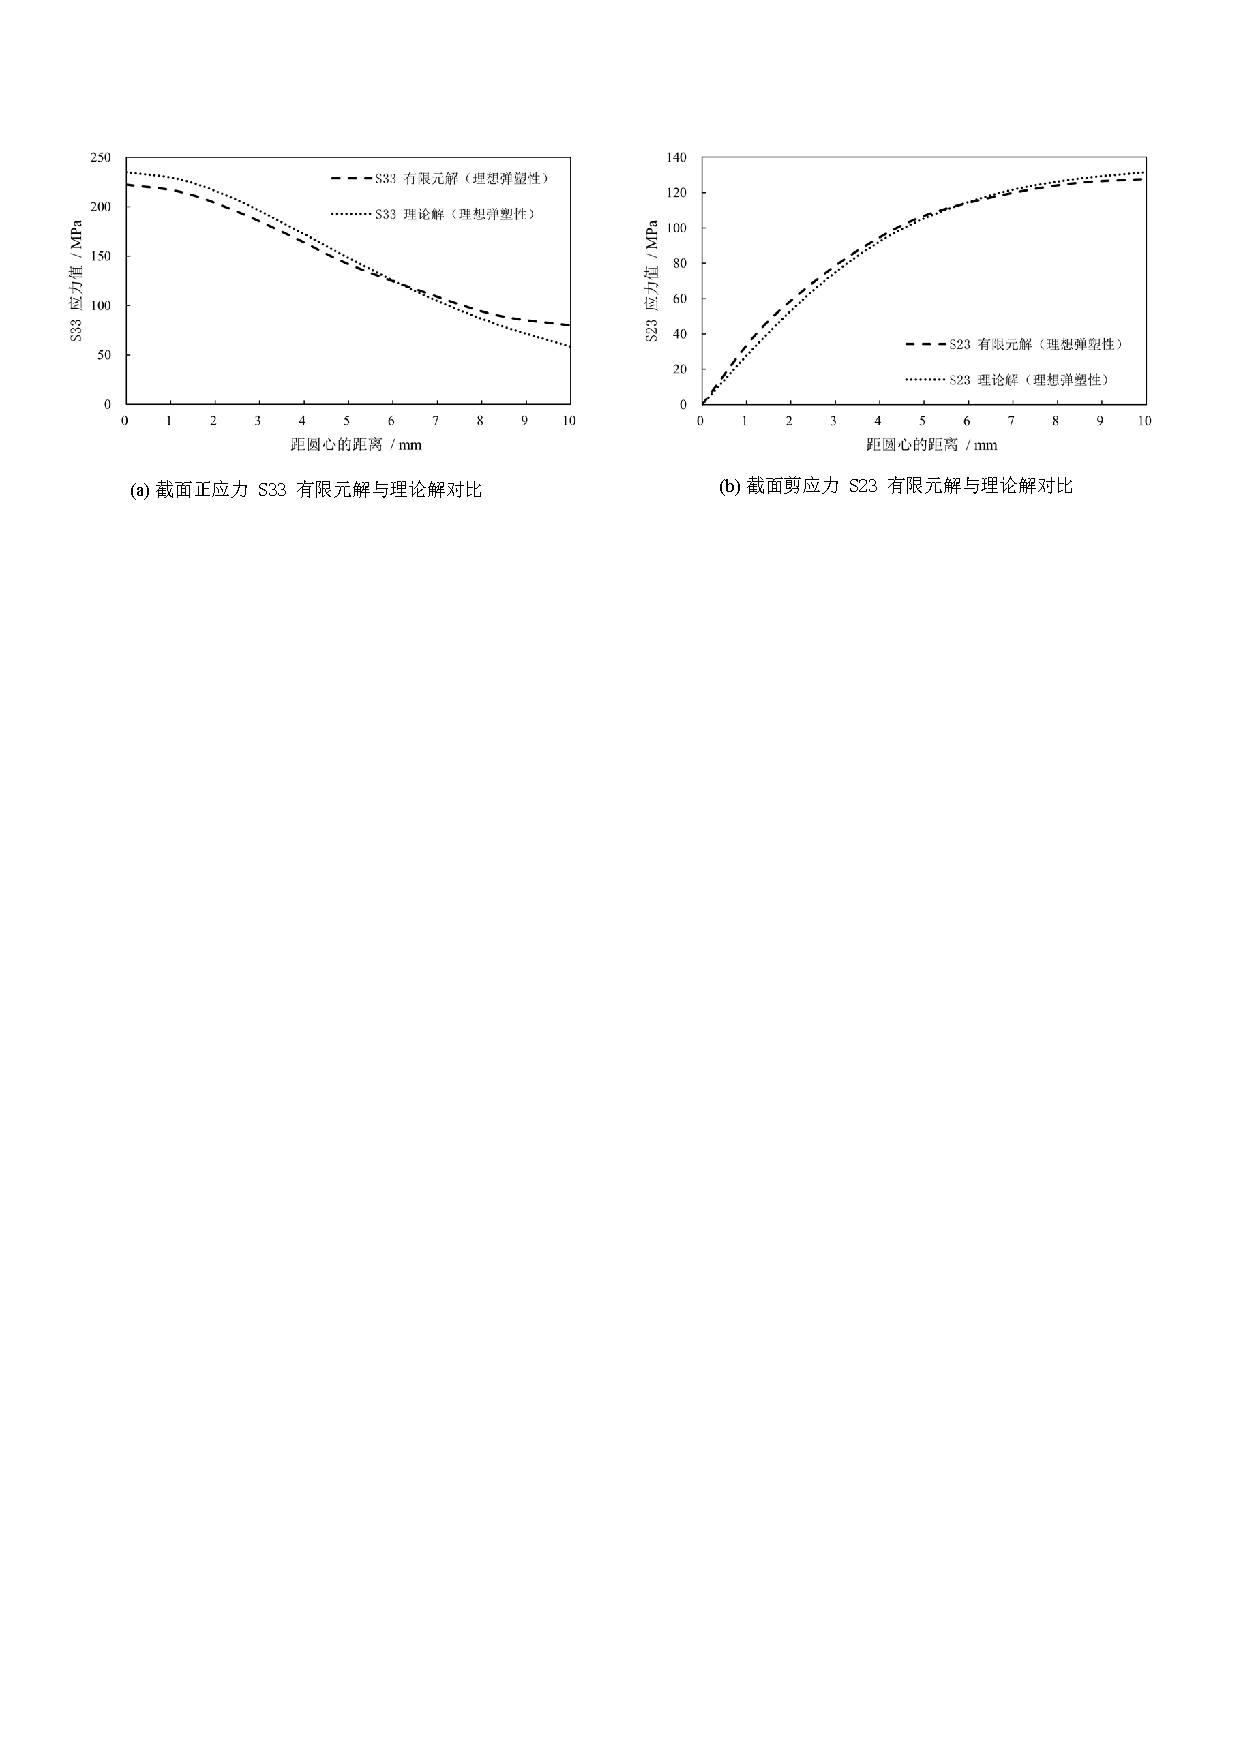
\includegraphics[width=1\textwidth]{1.pdf}
    \caption{理想弹塑性圆杆数值解与解析解对比}
    \label{fig:ideals3323}
\end{figure}






